\documentclass[11pt]{article}
\usepackage{array,booktabs,arydshln,xcolor}
\usepackage{tikz}
\usetikzlibrary{arrows}
\usetikzlibrary{patterns.meta}
\usetikzlibrary{decorations.pathreplacing}
\usetikzlibrary{decorations.markings,fpu}
\usetikzlibrary{decorations.pathmorphing}
\usepackage{amsmath}

\newcommand{\e}{\varepsilon}

\begin{document}

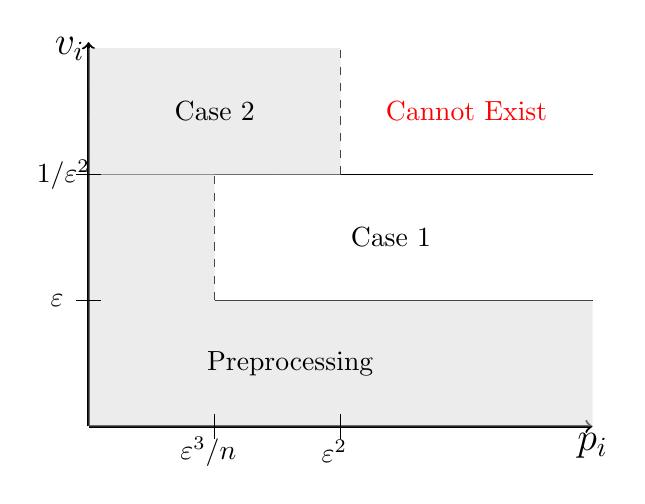
\begin{tikzpicture}[scale=0.8]

\pgfmathtruncatemacro{\casesL}{2};
\pgfmathtruncatemacro{\totalL}{8};

\tikzset{mycolor/.style={fill=gray!30, opacity=.5}}


%Draw horizontal lines
\draw[->, thick] (0,0)--(0,\totalL-1.9) node[]{};
\draw[-] (2,2)--(\totalL,2) node[]{};
\draw[-] (0,4)--(\totalL,4) node[]{};

%Draw vertical lines
\draw[-, dashed] (\casesL,2)--(\casesL,4) node[]{};
\draw[->, thick] (0,0)--(\totalL,0) node[]{};
\draw[-, dashed] (2*\casesL,4)--(2*\casesL,6) node[]{};



%Draw mlkies inside triangle

%Fill shapes with color
\fill[mycolor] (0,0)--(0,4)--(2,4)--(2,2)--(\totalL,2)--(\totalL,0);
\fill[pattern={Lines[angle=45, distance=6mm, line width=13mm, xshift=5mm]}, pattern color=gray!30,opacity=.5] (0,4)--(0,6)--(4,6)--(4,4);

\node[] at (-0.5,2) {$\varepsilon$};
		\draw[-] (-0.2, 2) --(0.2,2);

  		\node[] at (-0.4,4) {$1/\e^2$};
		\draw[-] (-0.2, 4) --(0.2,4);

\node[] at (-0.3,\totalL-2) {{\Large $v_i$}};
\node[] at (\totalL,-0.3) {{\Large $p_i$}};
		
\draw[-] (\casesL, -0.2) -- (\casesL, 0.2);
\node[] at (\casesL-0.1,-0.4) {$\e^3/n$};

\draw[-] (2*\casesL, -0.2) -- (2*\casesL, 0.2);

\node[] at (2*\casesL-0.1,-0.4) {$\e^2$};
%Cases
\node[] at (0.4*\totalL,1) {Preprocessing};
\node[] at (0.12*\totalL,3) {};
\node[] at (0.6*\totalL,3) {Case 1};
\node[] at (0.25*\totalL,5) {Case 2};
\node[] at (0.75*\totalL,5) {\color{red}{Cannot Exist}};

\end{tikzpicture}

\end{document}